\section{From the Nonlinear Plant to Executable Predictors}
\label{app:descriptor-bridge}
\newcommand{\BridgeDerivativeError}{3.91\times10^{-8}}
\newcommand{\BridgeTerminalError}{4.52\times10^{-13}}


The reduction in the method is checked against the implemented plant,
rather than a separate classical-machine example. This development
diagnostic uses the fixed initial state and parameter vector, before
prefix fitting, with 192 native variables: 114 differential and 78 algebraic.
It does not rerun the conditional bank or estimate an event from PMUs.

\subsection{Mass Normalization and Derivative Checks}
Write the native residual as
\begin{equation}
 M_d\dot x=F_q(x,z,a),\qquad 0=G_q(x,z,a),
\end{equation}
with constant nonsingular differential mass block $M_d$. At the same
differential reference $\bar x$ in each topology, solve
$G_q(\bar x,\bar z_q,0)=0$. Automatic differentiation of the assembled
network gives the blocks used in
\begin{align}
 Z_x&=-G_z^{-1}G_x,&Z_a&=-G_z^{-1}G_a,\nonumber\\
 A_q&=M_d^{-1}(F_x+F_zZ_x),&
 B_q&=M_d^{-1}(F_a+F_zZ_a),\nonumber\\
 c_q&=M_d^{-1}F_q(\bar x,\bar z_q,0),&
 C_q&=H_x+H_zZ_x,\nonumber\\
 D_q&=H_a+H_zZ_a.
\end{align}
Thus the main text's $f_q$ is the mass-normalized differential field.
The reference is fixed; a moving reference would additionally contribute
$-\dot{\bar x}$ and require consistent state and output recentering.
Here $H_q$ first selects rectangular bus voltages. Topology-specific
terminal stamps and polar derivatives form the PMU observations.
The load input $a$ scales the bus-7 P/Q setpoints together. Because its
load law is constant impedance, this is not a prescribed change in
instantaneous consumed power.

An independent numerical reconstruction of all four reduced operators
agrees to $4.3\times10^{-14}$ in maximum absolute entry error.
Centered directional checks against the native residual and consistent
nonlinear algebraic solves have maximum relative discrepancy
$\BridgeDerivativeError{}$, below the fixed $10^{-5}$ gate. These checks
cover the intact network and line 23--24 open. They establish local
derivative consistency, not accuracy for a finite excursion.
The algebraic Jacobian condition numbers are approximately 2109 and 2112
in the native scaling; neither value is a coordinate-invariant margin.

\subsection{Open-Loop Trajectories and Observation Coordinates}
Six new 12-s nonlinear trajectories use the same initial condition:
normal, bus-7 setpoint changes of $\pm1\%$ and $\pm10\%$ from 2 to 6\,s,
and line 23--24 open from 2 to 3\,s. All solves succeed. Samples include
both 0 and 12\,s; reports at switches use the post-switch algebraic state
and preserve the differential state. Terminal predictions at the eight
declared PMUs match the native current observables to
$\BridgeTerminalError{}$ pu, retaining orientation, transformer stamps
and the provisional bus-5 terminal assignment.

The reduced models start at zero deviation and propagate by an augmented
matrix exponential at 30 reports/s. They know the event times, location
and magnitude. No measured state correction, noise, covariance adjustment
or parameter fit is applied. At restoration, the state carries forward
and the nominal operators resume. The comparison therefore tests the
construction and its finite-excursion error; it does not measure source
attribution or the accuracy of the augmented conditional bank.

\begin{table}[t]
\centering\small
\caption{Open-loop errors at eight PMUs. Relative complex-voltage RMSE is normalized by the nonlinear event-response RMS; magnitude and phase errors use the first-order polar observation during recovery.}
\label{tab:descriptor-bridge}
\begin{tabular}{lrrrr}
\toprule
&\multicolumn{2}{c}{Complex error (\%)}&\multicolumn{2}{c}{Polar RMSE after OFF}\\
Event&ON&Recovery&$|V|$ (pu)&$\theta$ (deg)\\
\midrule
Load $+1\%$&0.72&1.48&$1.82\!\times\!10^{-8}$&0.0012\\
Load $-1\%$&0.72&1.48&$1.82\!\times\!10^{-8}$&0.0012\\
Load $+10\%$&7.14&14.82&$1.82\!\times\!10^{-6}$&0.1189\\
Load $-10\%$&7.17&14.89&$1.82\!\times\!10^{-6}$&0.1193\\
Line 23--24&17.97&30.70&$7.78\!\times\!10^{-4}$&3.1910\\
\bottomrule
\end{tabular}
\end{table}


For $\hat V=\bar V+\Delta V$, distinguish applying an exact polar
conversion to an approximate complex voltage from linearizing the polar
observation itself:
\begin{align}
 \widehat{|V|}&=|\bar V|+
 \Re\!\left(\Delta V\frac{\bar V^*}{|\bar V|}\right),\nonumber\\
 \hat\theta&=\arg\bar V+\Im(\Delta V/\bar V).
 \label{eq:bridge-polar}
\end{align}
The phase expression is in radians. Current channels use the same
derivatives at their nonzero reference currents, with the declared
terminal polarity and instrument gains. Both maps have the same local
derivative, but differ over a finite excursion. For example,
$\Delta V=\mathrm j\bar V\epsilon$ describes a phase tangent.
Taking its exact magnitude yields $|\bar V|\sqrt{1+\epsilon^2}$,
an artificial second-order magnitude rise. The linearized magnitude
correctly has zero first-order response. Figure~\ref{fig:descriptor-bridge}
shows why a small-signal complex-voltage approximation should not be
interpreted as an exact finite-rotation phasor.

\begin{figure*}[t]\centering
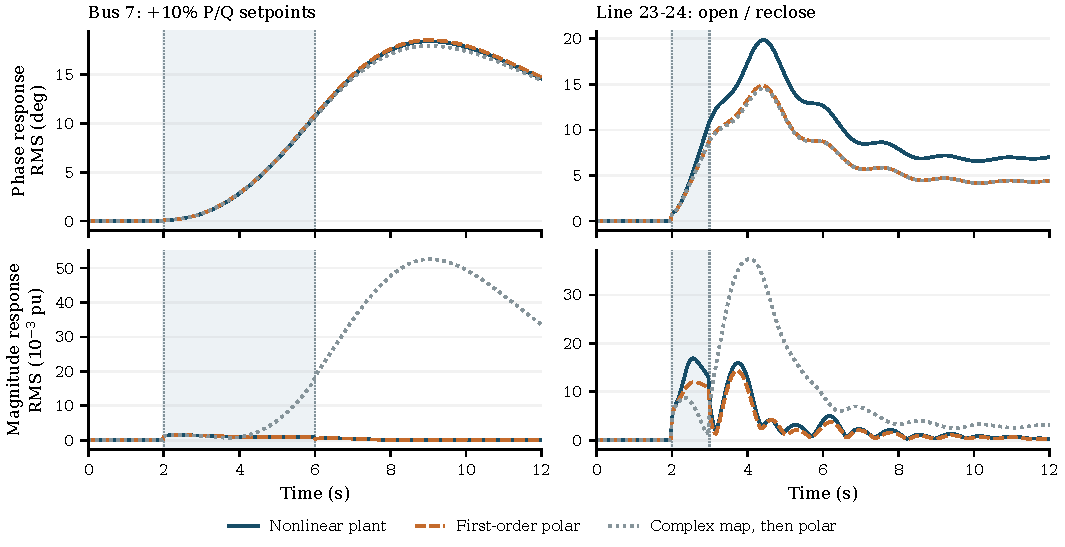
\includegraphics[width=.98\textwidth]{figures/generated/descriptor_bridge.pdf}
\caption{Open-loop predictions from the actual plant derivatives, with
known intervention times and no filtering. Curves are RMS deviations from
the matching normal trajectory over eight PMUs, not RMSE; shaded intervals
mark the active intervention. Solid: nonlinear plant. Dashed: reduced
dynamics with first-order polar observations. Dotted: reduced complex
voltage followed by exact polar conversion. The latter creates a large
spurious magnitude response during load recovery. The line case retains
a phase error with either map. Table~\ref{tab:descriptor-bridge} reports
errors for both load signs and magnitudes.}
\label{fig:descriptor-bridge}
\end{figure*}

Table~\ref{tab:descriptor-bridge} separates complex-voltage error from
the polar observation errors. Recovery means 6--12\,s for loads and
3--12\,s for the line, including the restored report. Reducing the load
step by ten reduces its absolute complex-voltage error by about one
hundred. This is consistent with local first-order accuracy in these
trajectories, not a global approximation bound. The line's recovery phase
error remains about 3.19 degrees with first-order polar observations;
correct derivatives do not remove finite-event model mismatch.

The reproducible outputs also retain separate magnitude, phase, frequency
and ROCOF errors for all 47 admitted coordinates. One comparison applies
the same robust causal phase estimator to both phasor trajectories;
another uses first-order polar channels and the predictor's ordinary
21-report polynomial fit. Their frequency and ROCOF errors include
different observation approximations and are not interchangeable.
These six deterministic cases have no independent statistical replicates.
They add a construction check and an explicit approximation limit, not
a Hamiltonian, graph-learning or adaptive-detection accuracy claim.
